\title{CS 378: Concurrency: Project Report}
\author{
        Sohaib Faruqi (sjf998) \\
        Department of Computer Science\\
        UT Austin
}
\date{\today}

\documentclass[9pt]{article}
\usepackage{graphicx}
\usepackage[margin=1.2in]{geometry}
\usepackage{comment}
\usepackage{hyperref}

\begin{document}
\maketitle

Note: code can be found at \url{https://github.com/sjf25/gpu-genetic-algorithm}

\section{Project Goals}
The goal of this project was to use CUDA to speed up genetic algorithms. In particular, the hope was to use CUDA to improve the selection, crossover, and mutation steps. I measured speedup with two different problems: Vertex Cover and MaxOne.

\section{How To Run}
Note: must be run on CUDA capable machine. First run ``make all". Then run the executable in the ``bin" folder with the following flags:
	\begin{itemize}
		\item -{}-input - name of input file (only for vertex cover problem)
		\item -{}-pop-size - size of the population (required)
		\item -{}-func-evals - number of function evaluations (func-evals/pop-size = number of iterations) (required)
		\item -{}-run-mode - mode to run in (either ``cuda" or ``seq") (required)
		\item -{}-problem - which problem to run (either ``vercov" or ``maxone") (required)
		\item -{}-num-runs - number of runs of the genetic algorithm (required)
		\item -{}-maxone-len - length of the bitarray (only for the maxone problem)
	\end{itemize}

\section{Background}
	\subsection{Genetic Algorithms}
		The idea is to try and come up with as good of a solution as
possible to some optimization problem. In genetic algorithms, each member is represented as an array
of bits. The population consists of members. The population changes each generation/iteration, using
the best solutions of the previous generation to create new members. The fitness function evaluates
how “good” of a solution a member is. The fitness function is dependent on the problem, so I should be
able to test my project on different optimization problems by changing the fitness function. The steps of
a genetic algorithm are as follows:
		\begin{enumerate}
			\item initalize population
			\item selection
			\item crossover
			\item mutation
			\item if not done, go back to step 2
		\end{enumerate}
	\subsection{Vertex Cover} The goal is to find the smallest set of vertices such that every edge in the graph has at least one end in the set.
	\subsection{Graph Density} Graph density,$D$, is defined as $D=\frac{2|E|}{|V|(|V|-1)}$. This is used to generate random graphs to test vertex cover.
	\subsection{MaxOne} The goal is to maximize the 1s in the member's bitarray. The optimal solution is just to have every element of the bitarray be 1. However, the genetic algorithm doesn't ``know" this, so it is a good problem to see if the algorithm is working and has an inexpensive fitness function.

\section{Design Choices}
The idea to use the vertex cover problem came from a paper by Khuri and B{\"a}ck titled ``An evolutionary heuristic for the minimum vertex cover problem" (which can be found at \url{https://www.researchgate.net/profile/Sami_Khuri/publication/2581134_An_Evolutionary_Heuristic_for_the_Minimum_Vertex_Cover_Problem/links/0912f5087009852297000000.pdf}).\\

I found the maxone problem on various places when reading up on genetic algorithms. I decided to use the maxone problem because it seemed simple with a inexpensive fitness function. I also chose it because the optimal solution for any length is known (bitarray of all ones) so it was good to test if the genetic algorithm was working.\\

I decided to use a roulette selection. This is because in my readings, fitness proportionate selection seemed to be the most commonly used and roulette selection seemed like the most common fitness proportionate selection that was reasonable to implement. I decided to use two-point crossover because that is what the paper by Khuri and B{\"a}ck used. In addition, I chose to used a mutation rate of $1/|V|$ where $|V|$ is the number of vertices when doing the vertex cover problems since that is what Khuri and B{\"a}ck did. I also used the same crossover rate and a similar fitness function for vertex cover as the paper.\\

Another important design choice was to NOT optimize the fitness functions in the CUDA version by computing them in parallel. It would have been possible to do this because both problems chosen consisted of calculating a penalty for each ``bit" and summing these penalties together. The reason I chose not to do this is because I wanted to see if I could speedup the steps of the genetic algorithm itself, not the fitness functions. So I thought it would be fair to have the fitness functions as close to idential for the sequential and CUDA version.\\

I also chose to have the fitness function be one that should be maximized instead of minimized. I did this because it made the roulette selection easier to implement. Since the paper by Khuri presented a fitness function to be maximized, I did 1 divided by it (i.e. the reciprocal). This was safe to do because the only time their fitness function could be zero is when $|V| = 0$.\\

For the CUDA version, I decided for the number of blocks to be the number of runs desired and the number of threads per block to be the population size. I did this because it is often necessary to rerun a genetic algorithm multiple times since it can become stuck in local minima/maxima. So the best fitness of multiple runs is taken to be the overall best solution.

\section{Limitations}
When the number of runs is limited to 1, the CUDA version only becomes faster than the sequential version when there are many (seems to be a couple hundred) members. However, in the readings I did, it doesn't seem common to use hundreds of members in the population.

\section{Implementation Tricks/Hacks}
I ran into the situation where I needed a parallel scan both to sum the fitness and find the max fitness, but only within one block. So I implemented a general templated-function that takes in an operator and performs the parallel scan. I also used a boolean array so threads would know when they could perform some operations (for example, it's not neccesary to wait for every thread to finish selection before crossover. A thread just needs to wait for the thread it's crossing over with).

\section{Evaluation}
It seems like when the number of runs of the genetic algorithm was limited to 1, the CUDA version was slower than the sequential version until there were a couple hundred members. I believe this is because the inital cost of CUDA (such as copying memory to and from the device, launching kernels, etc.) was higher but it scaled better as the number of threads increased.\\

\begin{figure}[t]
  \centering
  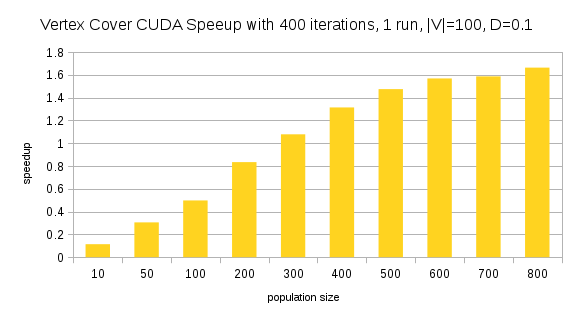
\includegraphics[width=.9\textwidth]{vc_change_pop.png}
  \caption{Speedup for Vertex Cover, varying population size}
  \centering
  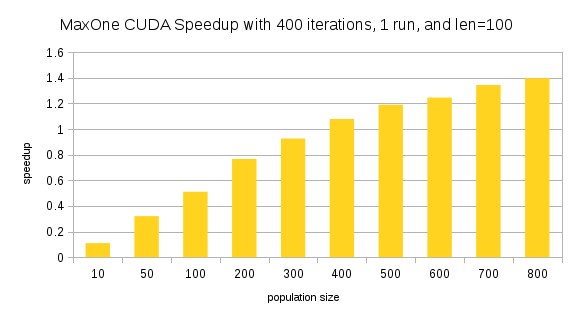
\includegraphics[width=.9\textwidth]{maxone_change_pop.png}
  \caption{Speedup for MaxOne, varying population size}
\end{figure}

The CUDA version seemed to do much better than the sequential version when the algorithm was run multiple times. This is because in the CUDA code, it was as simple as increasing the number of blocks while in the seequntial version algorithm had to be repeated sequentially.\\

\begin{figure}[t]
  \centering
  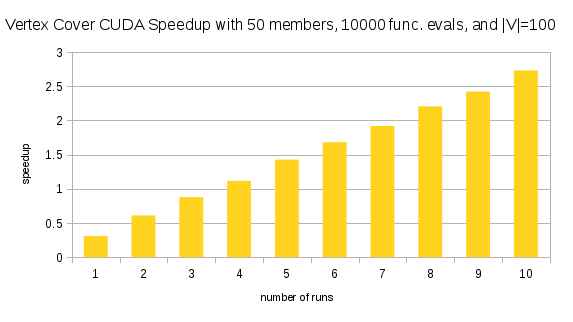
\includegraphics[width=.9\textwidth]{vc_change_runs.png}
  \caption{Speedup for Vertex Cover with graph density = 0.1, varying the number of runs}
  \centering
  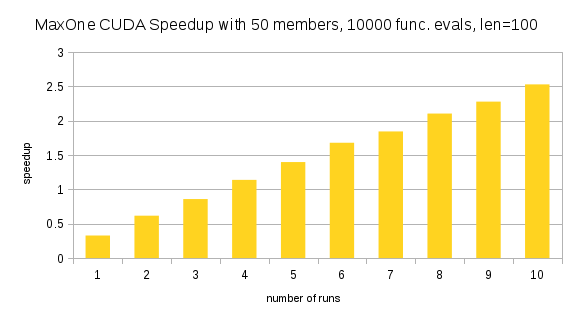
\includegraphics[width=.9\textwidth]{maxone_change_runs.png}
  \caption{Speedup for MaxOne, varying the number of runs}
\end{figure}

I also replicated the experiment in the paper by Khuri with both the sequential version and CUDA version. When there were 100 vertices, the speedup was as high as 23 times more than the sequential. I was unable to obtain a speedup graph for the part of the experiment where 200 vertices were used, because the sequential version was too slow to finish.\\

Overall, the CUDA version is better when there are hundred of members in the population and/or multiple runs of the algorithm are being done.

\begin{figure}[t]
  \centering
  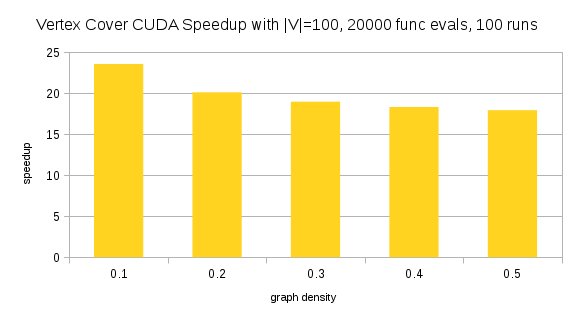
\includegraphics[width=.9\textwidth]{khuri_exper_100.png}
  \caption{Speedup for Vertex Cover experiment in paper, with $|V|=100$. Unable to do for $|V|=200$ because sequential takes \textbf{very} long to finish}
\end{figure}

\section{Time Spent}
About 30-40 hours.

\bibliographystyle{abbrv}
%\bibliography{main}

\end{document}
This is never printed
